\chapter{Systematic uncertainties}

\label{ch:systematics}

Every cross-section measurement, such as the one presented here, inherently carries uncertainties crucial for understanding the reliability and precision of the reported result. These uncertainties can be divided into two categories: statistical and systematic.

The statistical uncertainty essentially accounts for the fact that a cross-section measurement is a counting experiment with a finite number of counts. Specifically, this work involves counting antineutrino interactions in bins of $p_{\text{T}}$ and Bjorken~$x$. Each count, i.e. the observed interaction, originates from an underlying Poisson probability distribution. Therefore, the statistical uncertainty of a given bin with $N$ events corresponds to $\sqrt{N}$. 
% p24: https://indico.cern.ch/category/6015/attachments/192/629/Statistics_introduction.pdf
%observed number of events will be Poisson distributed a the normal approximation to the Poisson distribution. 
%Note that the statistical uncertainty of the unfolded distribution is corrected to account for the finite statistics of the unfolding matrix as described in Section~\ref{sec:migration_unfolding}. 

In contrast, systematic uncertainties in this measurement describe the accuracy with which the cross-section can be measured, taking into account the limitations of the MINERvA and MINOS detectors and reconstruction, as well as the understanding of the incident antineutrino beam and its interactions with nuclei. MINERvA uses the underlying simulation to estimate systematic uncertainties in reported cross-section results via the multiverse method \cite{MAT_Messerly_2021}, which has already been mentioned in Chapters~\ref{ch:minerva} and \ref{ch:dataAsimulation} with respect to flux modelling. The simulation with nominal values for all parameters, as described in Chapter~\ref{ch:dataAsimulation}, is referred to as the central value~(CV). A~systematic universe is then a simulation sample in which one or more input parameters are varied within their associated uncertainties. 

As discussed, the antineutrino flux, due to its complex modelling, necessitates the multiverse approach to allow simultaneous variations of multiple parameters. However, most systematic uncertainties have relatively simple underlying models and are typically evaluated by considering two universes where a parameter is shifted by $\pm 1 \sigma$, with $\sigma$ representing the parameter's uncertainty. The magnitude of the uncertainty in each bin is then given by the spread of these two universes, i.e. the average difference between each universe and the CV in that bin. All systematic universes are propagated throughout the analysis.

\begin{figure}[t!]%
    \centering
    \vspace{-5pt}
   {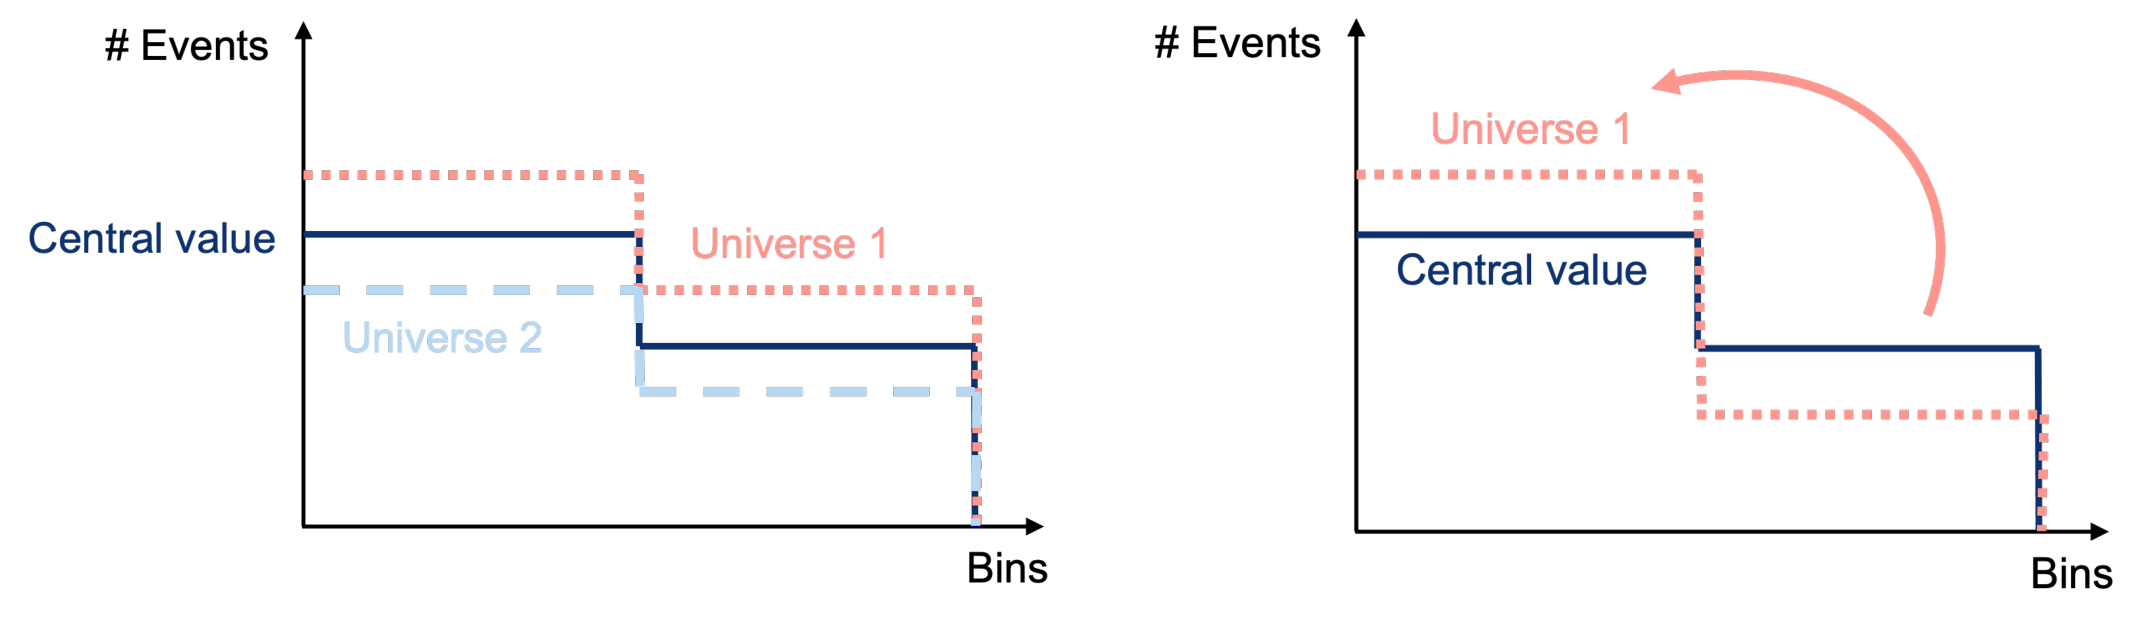
\includegraphics[width=0.9\textwidth]{08systematics/figures/systematicShifts.pdf} }%
    \caption{Illustration of two different effects a systematic universe can have on an event---a normalisation-like shift (left) and a bin-by-bin shift (right). }%
    \label{fig:sysShifts}
\end{figure}

Conceptually, there are two effects a systematic universe can have on an event: a~normalisation-like shift and a bin-by-bin shift, as illustrated in Figure~\ref{fig:sysShifts}. Normalisation-like shifts represent uncertainties that affect the weight of an event in a given bin, such as those from interaction models. In contrast, bin-by-bin uncertainties impact the kinematic variables, causing bin-to-bin migration, and represent most detector systematics. 

Figure~\ref{fig:mcSimulationFracUnc_t5lead_pTx} shows an example of the fractional uncertainty\footnote{Fractional uncertainty error band represents the uncertainties relative to the CV, i.e.~uncertainty/CV.} on the simulation for target~5 lead both in $p_{\text{T}}$ and Bjorken~$x$ at the event rate level. Appendix~\ref{ch:appendix_sysUncertainties} includes the corresponding breakdown of uncertainties for the scintillator tracker. Related sources of uncertainties are grouped together in one error band and will be discussed individually later with respect to the reported cross-section. The individual systematic errors within these groups are constructed by extracting the square root of diagonal entries (variances) of their corresponding covariance matrices. 

An element of the covariance matrix relating two bins $i$~and $j$ can be calculated as
\vspace{-7pt}
\begin{equation}
    \label{eq:covariance}
    %\vspace{-10pt}
    \text{cov}_{ij} = \frac{1}{N-1}\sum_{n=1}^{N}(x_{n, i} - \bar{x}_i)(x_{n, j} - \bar{x}_j)
    \hspace{3pt},
    \vspace{5pt}
    %\text{cov}_{ij} = \frac{\sum_{n=1}^{N} (x_{n, i} - \bar{x}_i)(x_{n, j} - \bar{x}_j)w_n}{\sum_{n=1}^{N} w_n}\hspace{3pt},
\end{equation}
where $N$ represents the total number of universes, $x_n$ is the bin content of a given bin in the universe $n$, and $\bar{x}$ is the mean of all the universes in that bin.  Note that the off-diagonal terms of the covariance matrix are retained and used in comparisons with various other antineutrino generators with different interaction models in Chapter~\ref{ch:results} to account for bin-to-bin correlations.~The error band grouping related sources of uncertainty in each bin is then calculated as the square root of the sum of the diagonal elements of all relevant individual covariance matrices. The total error band is calculated the same way but also includes the statistical uncertainty.

%In this way, the variance of each bin is added in quadrature as expected for uncorrelated uncertainties.

\begin{figure}[t!]%
    \vspace{-7pt}
    \centering
   {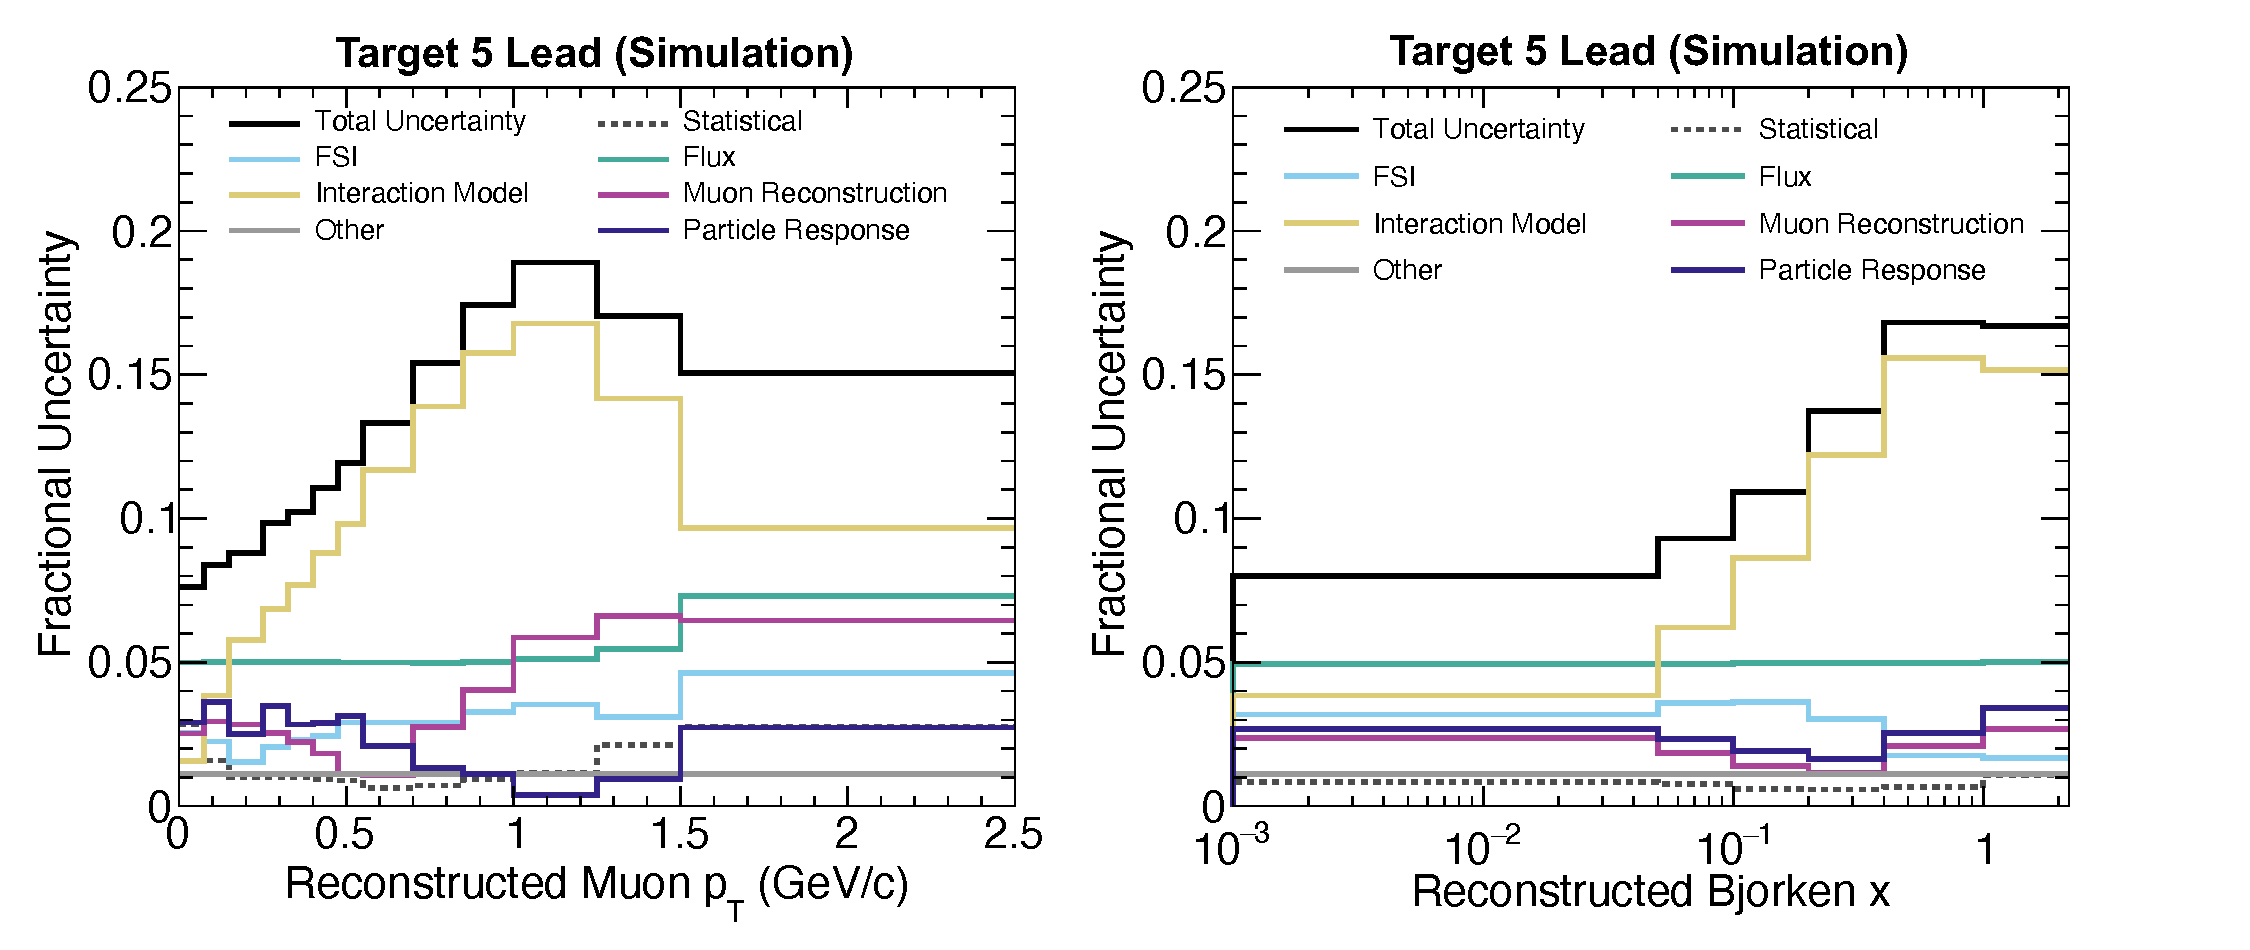
\includegraphics[width=1\textwidth]{08systematics/figures/mcSimulationFracUnc_t5lead_pTx.pdf} }%
    \caption{Fractional uncertainty breakdown for the simulated event rate in both $p_{\text{T}}$~(left) and Bjorken~$x$ (right) in target 5 lead.}%
    \label{fig:mcSimulationFracUnc_t5lead_pTx}
\end{figure}

The multiverse method enables independent cross-section analysis in each universe. While the systematic uncertainty is reported on the simulation at the event rate level, in the final cross-section result, MINERvA reports the systematic uncertainty on the data. This is due to the cross-section extraction steps outlined in Equation~\ref{eq:xsec1D}, i.e. background subtraction, unfolding, efficiency correction, and normalisation, where information from the simulation introduces systematic uncertainty to the data.

The (data) cross-section uncertainty for the differential cross-section on lead in $p_{\text{T}}$ and Bjorken~$x$ is presented in Figure~\ref{fig:crossSectionFracUnc_lead_pTx}. The individual error band categories are discussed in detail in the following sections.\enlargethispage{1\baselineskip} However, it is important to note that Figure~\ref{fig:crossSectionFracUnc_lead_pTx} illustrates a general trend observed across various materials for the last $p_{\text{T}}$ and Bjorken~$x$ bin. Specifically, the last $p_{\text{T}}$ bin, extending to the edge of the angular acceptance, leads to statistical fluctuations in the associated systematic uncertainty.~On the other hand, the last Bjorken~$x$ bin is significantly influenced by interaction model uncertainties since the simulation doesn't directly model this region at the nucleon level, as discussed previously. In the kinematic distributions (as opposed to fractional uncertainty plots), where the data carries the systematic uncertainty, the data points are represented with inner and outer error bars, corresponding to the statistical and total (statistical + systematic) uncertainty, respectively.



\begin{figure}[t!]%
    \centering
    \vspace{-7pt}
   {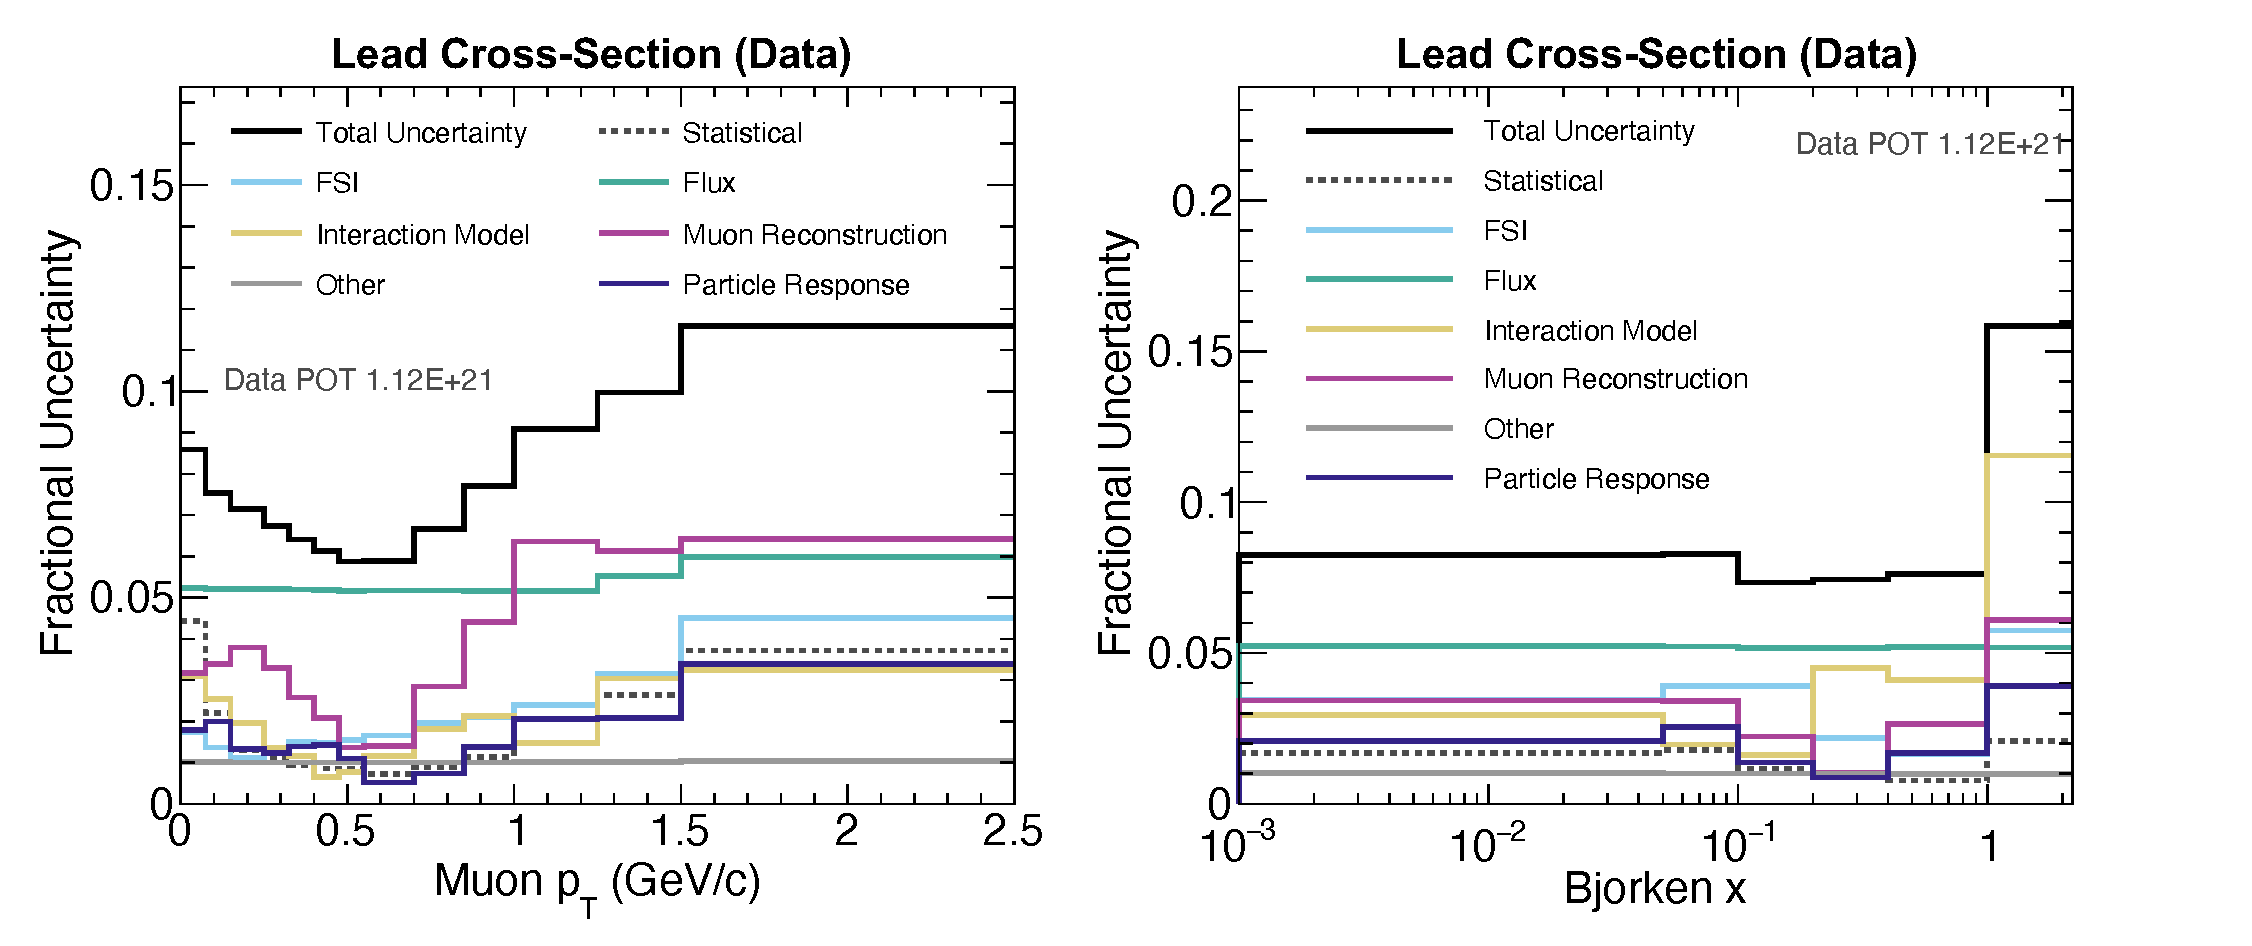
\includegraphics[width=1\textwidth]{08systematics/figures/crossSectionFracUnc_lead_pTx.pdf} }%
    \caption{Breakdown of the fractional uncertainties propagated to the lead differential cross-section in data in both $p_{\text{T}}$~(left) and Bjorken $x$ (right).}%
    \label{fig:crossSectionFracUnc_lead_pTx}
\end{figure}

\section{Flux}

Similarly to other cross-section analyses, the flux uncertainty represents the leading systematic uncertainty in this measurement as well\footnote{One of the primary reasons for reporting cross-section ratios is to cancel out the dominant flux uncertainty.}. The flux modelling and its associated uncertainties have been discussed in detail in Chapters~\ref{ch:minerva} and \ref{ch:dataAsimulation}. MINERvA's PPFX package \cite{AliagaSoplin:2016shs, Aliaga_2014} evaluates the flux uncertainty in 1000 systematic universes, where each universe represents an ensemble of systematic variations of underlying beam-focusing and hadron production parameters to account for their non-trivial correlations resulting from the fits described in Subsection~\ref{subsec:numiSim}.

In addition, MINERvA applies an \textit{in-situ} constraint combining measurements of (anti)neutrino-electron scattering and IMD \cite{Zazueta2023_PhysRevD.107.012001}, which significantly reduces the flux uncertainty in the antineutrino-dominated beam to about 5\% as evident from Figure~\ref{fig:crossSectionFracUnc_lead_pTx}. The \textit{in-situ} constraint assigns weights to the individual flux universes, with some being weighted much more than others, allowing for their ordering in terms of significance. Previous MINERvA studies have shown that, in most cases, the most significant 100 universes adequately sample the range of systematic variations \cite{fluxReorderingRobFine}. This allows for a reduction in computational power when evaluating the flux uncertainty at the cross-section measurement level, and is therefore used in this analysis. Note that the flux uncertainty in both $p_{\text{T}}$ and Bjorken~$x$, as shown in Figure~\ref{fig:crossSectionFracUnc_lead_pTx}, is flat since the cross-sections are differential.


\section{Antimuon reconstruction}

\begin{figure}[b!]%
    \centering
   {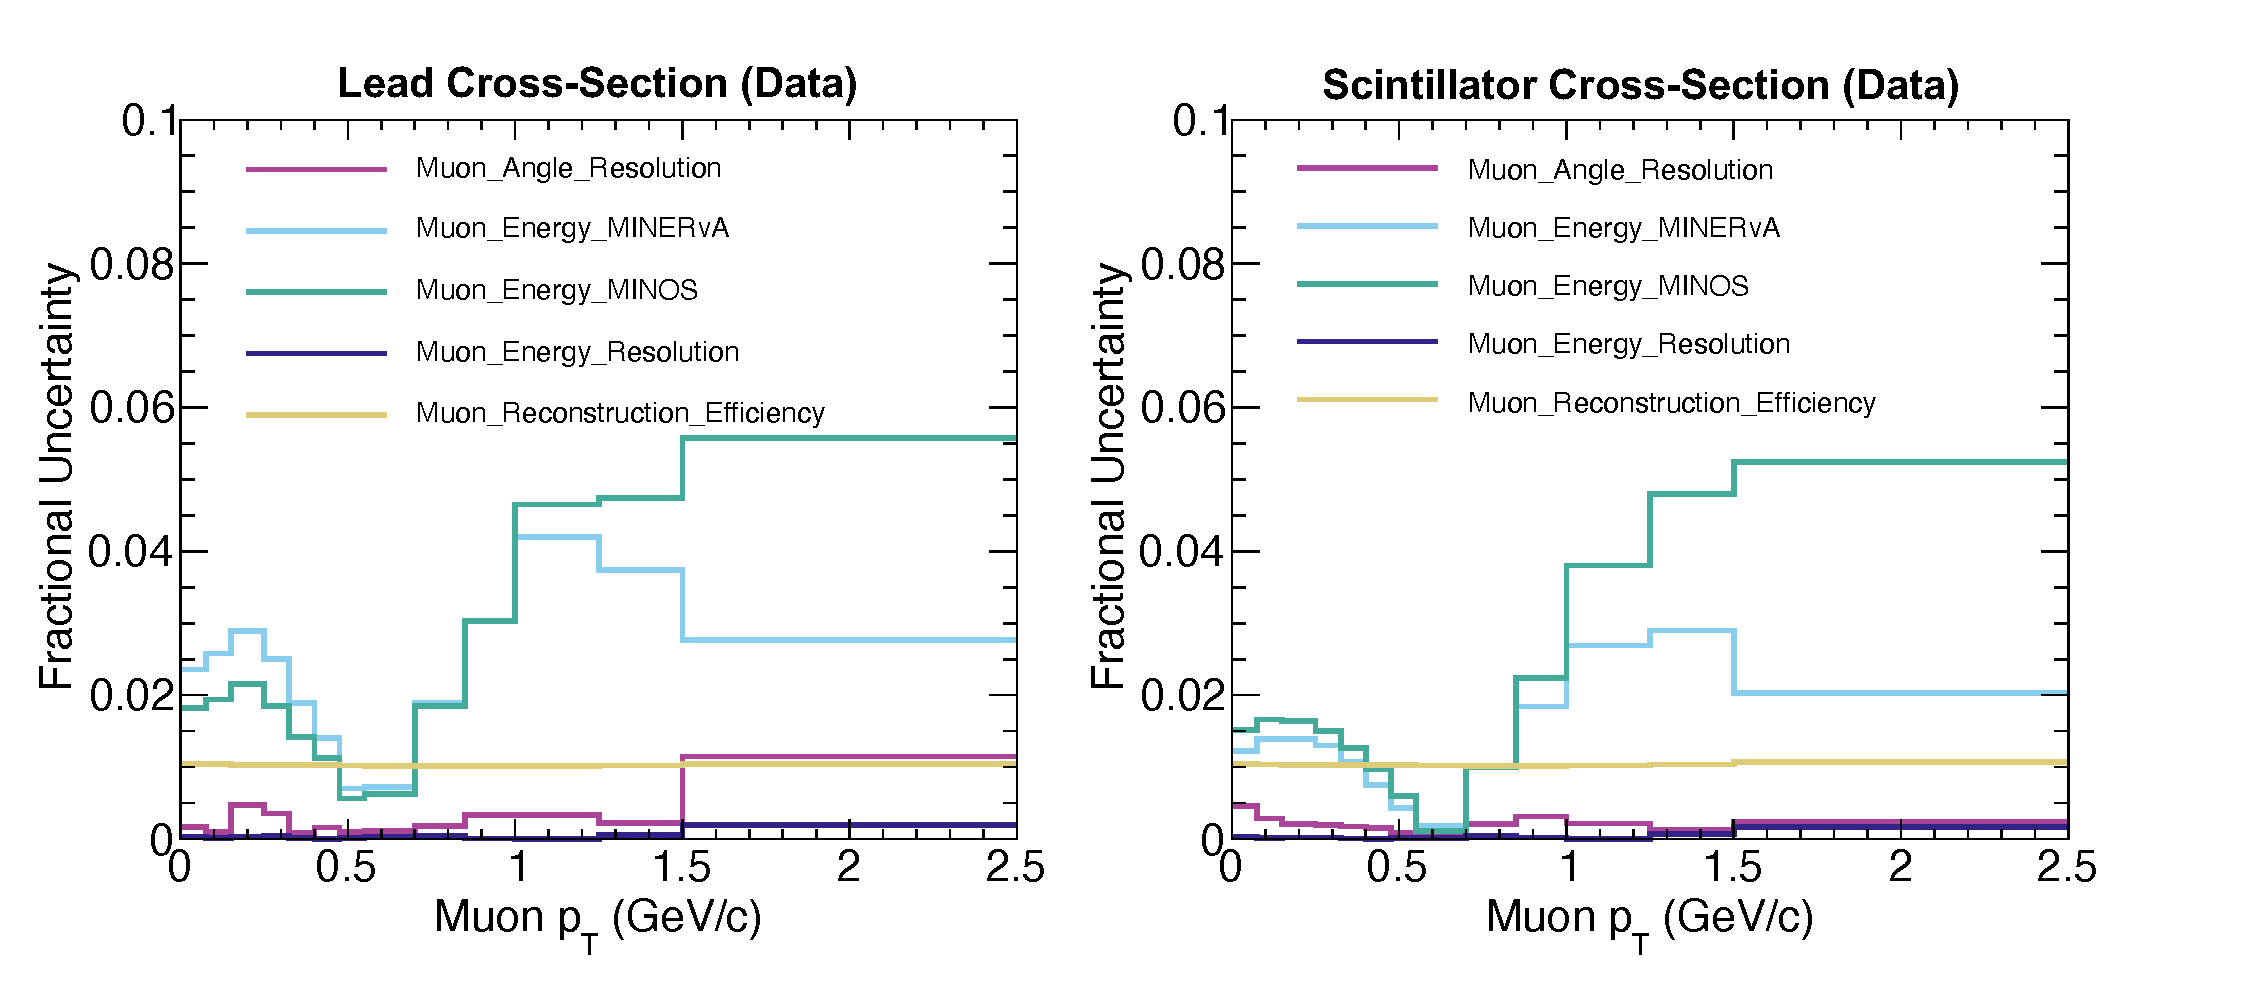
\includegraphics[width=1\textwidth]{08systematics/figures/muonReco_leadTracker_pT.pdf} }%
    \caption{Breakdown of various sources of uncertainty in the `Muon Reconstruction' error band in the lead (left) and scintillator (right) differential cross-section in data in $p_{\text{T}}$.}%
    \label{fig:muonReco_leadTracker_pT}
\end{figure}

The uncertainty related to antimuon reconstruction is the second-largest (third-largest) uncertainty in the  $p_{\text{T}}$ (Bjorken $x$) differential cross-section.\enlargethispage{1.5\baselineskip} Figure~\ref{fig:muonReco_leadTracker_pT} shows the error band broken down into the various sources of uncertainties for both lead and scintillator cross-sections in $p_{\text{T}}$, while the corresponding breakdown for Bjorken~$x$ is provided in Appendix~\ref{ch:appendix_sysUncertainties}. The $p_{\text{T}}$ breakdown is dominated by the uncertainty on the antimuon energy reconstruction in the MINERvA detector and MINOS spectrometer. The MINERvA uncertainty combines the 40~MeV (30~MeV) uncertainty on the energy deposits per unit length and the  17~MeV (11~MeV) material assay uncertainty for the passive target region (active tracker region)~\cite{Tice_PhysRevLett.112.231801}. The MINOS uncertainty comes from the~0.98\% uncertainty on antimuons reconstructed by range, and the~2.1\%~(3.2\%) uncertainty on antimuons with momenta above (below) 1~GeV reconstructed by curvature~\cite{Aliaga_2014}, as described in Chapter~\ref{ch:Reconstruction}.
% there is also material assay uncertainty 11 MeV shift vs 17 MeV

The flat reconstruction efficiency uncertainty band represents the uncertainty on the tracking efficiency of the MINOS spectrometer stemming from the antimuon energy- and beam intensity-dependent correction applied to the simulation to match the data, also discussed in Chapter~\ref{ch:Reconstruction}. The antimuon angle uncertainty encompasses the 2\% uncertainty on the reconstructed antimuon angle~\cite{Ziemer:2012ota}, and the 1~mrad antimuon angle bias coming from the uncertainty on the incoming antineutrino beam angle~\cite{Valencia-Rodriguez:2016vkf}. Finally, the uncertainty in antimuon energy resolution corresponds to 0.4\%~\cite{Bashyal:2021tzd} and quantifies any remaining antimuon energy resolution differences between the data and the simulation.


% muon track uncertainty https://lss.fnal.gov/archive/thesis/2000/fermilab-thesis-2012-62.pdf
% beam angle thing: https://www.osti.gov/biblio/1341804
% muon energy resoltion - I guess bercelie? or Bashyal?


\section{Interaction model}
% summary table for GENIE uncertainties:
% https://minerva-docdb.fnal.gov/cgi-bin/sso/RetrieveFile?docid=7451&filename=ReweightingSystematics.pdf&version=2

\begin{figure}[t!]%
    \centering
    \vspace{-7pt}
   {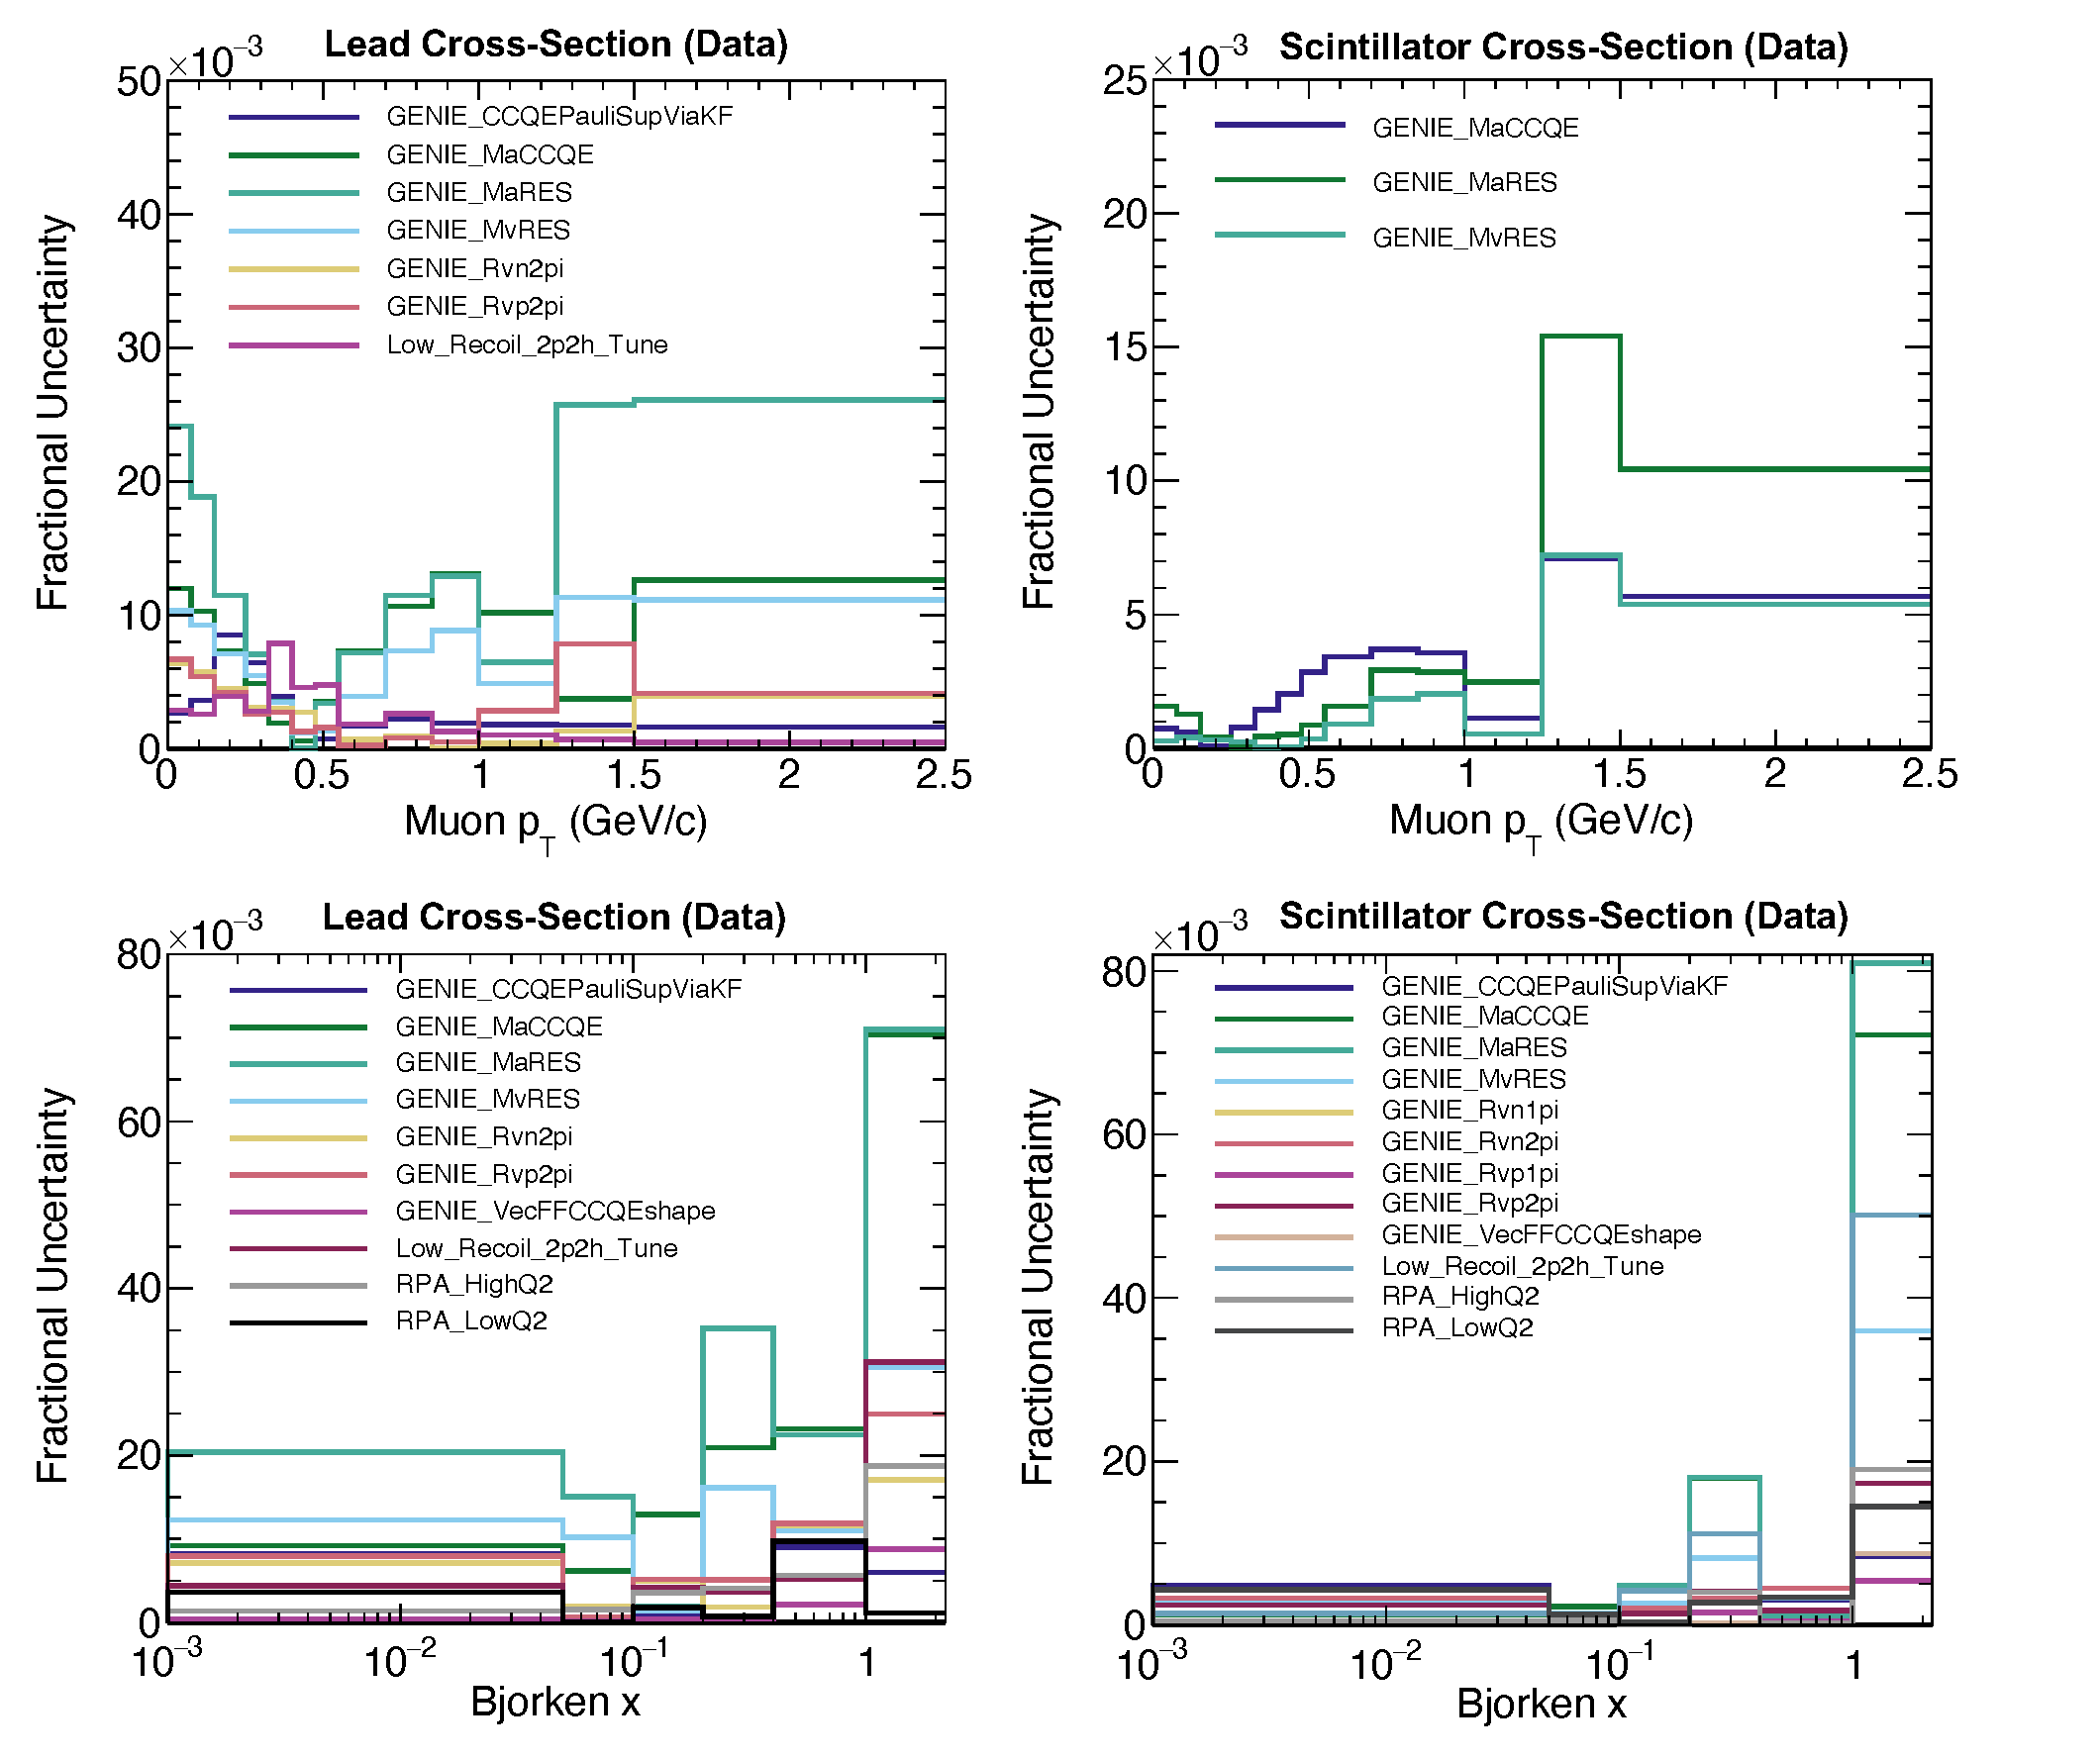
\includegraphics[width=1\textwidth]{08systematics/figures/intModel_t5Tracker_pTx.pdf} }%
    \caption{Breakdown of various sources of uncertainty in the `Interaction Model' error band of the differential cross-section in data, both in $p_{\text{T}}$ (top) and Bjorken $x$ (bottom) for lead (left panel) and scintillator (right panel), with contributions exceeding 0.5\%. Note the dominant contribution from the uncertainty on the resonant pion production axial mass.}%
    \label{fig:intModel_t5Tracker_pTx}
\end{figure}

The initial state and initial interaction models used in the simulation, described in detail in Chapter~\ref{ch:dataAsimulation}, have several parameters that adjust the probability of an interaction process occurring. The underlying uncertainties associated with these parameters in GENIE~\cite{genie_ANDREOPOULOS201087,genie_andreopoulos2015}, derived from previous experimental measurements, enable the construction of alternative universes to evaluate corresponding systematic uncertainties in the measurement. Some of these default uncertainties are constrained using MINERvA's measurements and re-analyses of other data. There are also additional uncertainties related to the previously discussed RPA and 2p2h implementations. All these uncertainties are combined in the `Interaction Model' error band, as shown in Figures~\ref{fig:mcSimulationFracUnc_t5lead_pTx} and~\ref{fig:crossSectionFracUnc_lead_pTx}.\enlargethispage{1\baselineskip}
% uncertainties on various parameters: GENIE source code
% https://github.com/GENIE-MC/Generator/blob/R-2_12_6/src/ReWeight
% https://indico.fnal.gov/event/11610/contributions/9102/

% info from: https://minerva-docdb.fnal.gov/cgi-bin/sso/RetrieveFile?docid=7451&filename=ReweightingSystematics.pdf&version=2
% https://github.com/MinervaExpt/MAT-MINERvA/blob/main/utilities/NSFDefaults.h
% Bercellie thesis and Rob Fine thesis
\begin{table}[t!]
    \centering
    \small
    \begin{tabularx}{1.0\textwidth}{c c L}
    \hline \\ [-1.5 ex]
    Error band & 1$\sigma$ & Description\\ [0.5ex] % inserts table %heading
    \hline
    \hline \\ [-2ex]
    CCQEPauliSupViaKF & $\pm30$\% & Modifies Pauli blocking at low $Q^2$ by adjusting momentum cutoff \\
    MaCCQE & +25\%/-15\% & CCQE axial mass (0.99 GeV/$c^2$) in the Llewellyn-Smith cross-section (shape and normalisation) \\
    MaRES & $\pm0.05$ GeV/$c^2$ & RES axial mass (0.94 GeV/$c^2$) in the Rein-Sehgal cross-section (shape and normalisation) \\
    MvRES & $\pm3$\% & RES vector mass (0.84 GeV/$c^2$) in Rein-Sehgal cross-section (shape and normalisation) \\
    Rvn1pi & $\pm4$\% & Strength of CC and NC 1$\pi$ production from non-resonant (Bodek-Yang) $\nu n$/$\bar{\nu}p$ interactions  \\
    Rvn2pi & $\pm50$\% & Strength of CC and NC 2$\pi$ production from non-resonant (Bodek-Yang) $\nu n$/$\bar{\nu}p$ interactions \\
    Rvp1pi & $\pm4$\% & Strength of CC and NC 1$\pi$ production from non-resonant (Bodek-Yang) $\nu p$/$\bar{\nu}n$ interactions \\
    Rvp2pi & $\pm50$\% & Strength of CC and NC 2$\pi$ production from non-resonant (Bodek-Yang) $\nu p$/$\bar{\nu}n$ interactions \\
    VecFFCCQEshape & BBBA~$\rightarrow$~dipole & CCQE vector form factor model change from BBBA to dipole (shape) \\
    \hline
    \end{tabularx}

    \caption{Description of various sources of uncertainty in the `Interaction Model' error band from Figure~\ref{fig:intModel_t5Tracker_pTx} with their corresponding 1$\sigma$ shifts.}
    \label{table:intModelUnc}
\end{table}

Figure~\ref{fig:intModel_t5Tracker_pTx} shows the uncertainties that contribute more than 0.5\% to the `Interaction Model' uncertainty band in the $p_{\text{T}}$ and Bjorken~$x$ differential cross-section in both lead and scintillator. A close-up of the scintillator breakdown in Bjorken~$x$ for the $x<1$ region is provided in Appendix~\ref{ch:appendix_sysUncertainties}. Overall, the error band is dominated by the resonant pion production axial mass uncertainty, which is expected given that resonant pion production is the dominant interaction channel in this analysis.~Additional notable contributions come from the uncertainty on the vector mass in resonant pion production and the axial mass in quasi-elastic scattering. All of these govern the cross-section shape and normalisation of their respective processes. Table~\ref{table:intModelUnc} lists and describes all GENIE parameter uncertainties contributing more than 0.5\%. Note that in comparison to the nominal uncertainties in GENIE, the uncertainty on $M_A^{\text{RES}}$ is constrained from the nominal 20\% to about~5\% by the reanalysis of the ANL/BNL deuterium bubble chamber measurements of single pion production~\cite{pion_Rodrigues_2016}, mentioned in Chapter~\ref{ch:dataAsimulation}. In addition, the uncertainties on the single-pion non-resonant production parameters are constrained from 50\% to 4\% using the same reanalysis. Fits~\cite{PhysRevD.74.014009} to pion production in electron-nucleon scattering~\cite{Tiator_2004} are also used to reduce the uncertainty on $M_V^{\text{RES}}$ from 10\% to 3\%.
% doc-db for vector mass uncertainty: https://minerva-docdb.fnal.gov/cgi-bin/sso/ShowDocument?docid=11567
% axial mass norminal uncertainty 20% of 

Furthermore, the uncertainty associated with the 2p2h model used in the MINERvA simulation, as described in Section~\ref{subsec:2p2h}, is assessed by varying the composition of correlated pairs of nucleons. This variation extends to the extremes of either exclusively proton-proton (neutron-neutron) pairs or exclusively neutron-proton pairs involved in the 2p2h process to construct the alternative universes~\cite{Gran2018_PhysRevLett.120.221805}. The RPA uncertainty is evaluated similarly by varying its implementation in the universes separately for the low-momentum and high-momentum transfer regions.\enlargethispage{1\baselineskip} The former comes from the comparisons against data for muon capture at low-momentum transfer, while the latter stems from the differences between the relativistic (implemented in the simulation CV) and the non-relativistic RPA calculation at high-momentum transfer~\cite{gran2017model}.

% 60% relativistic vs non-relativistic in high momentum - non-relativistic is higher
% data-driven  - 25\% normalisation difference

\section{FSI}
% FSI uncertainties description https://minerva-docdb.fnal.gov/cgi-bin/sso/ShowDocument?docid=7451
\begin{figure}[b!]%
    \vspace{-7pt}
    \centering
   {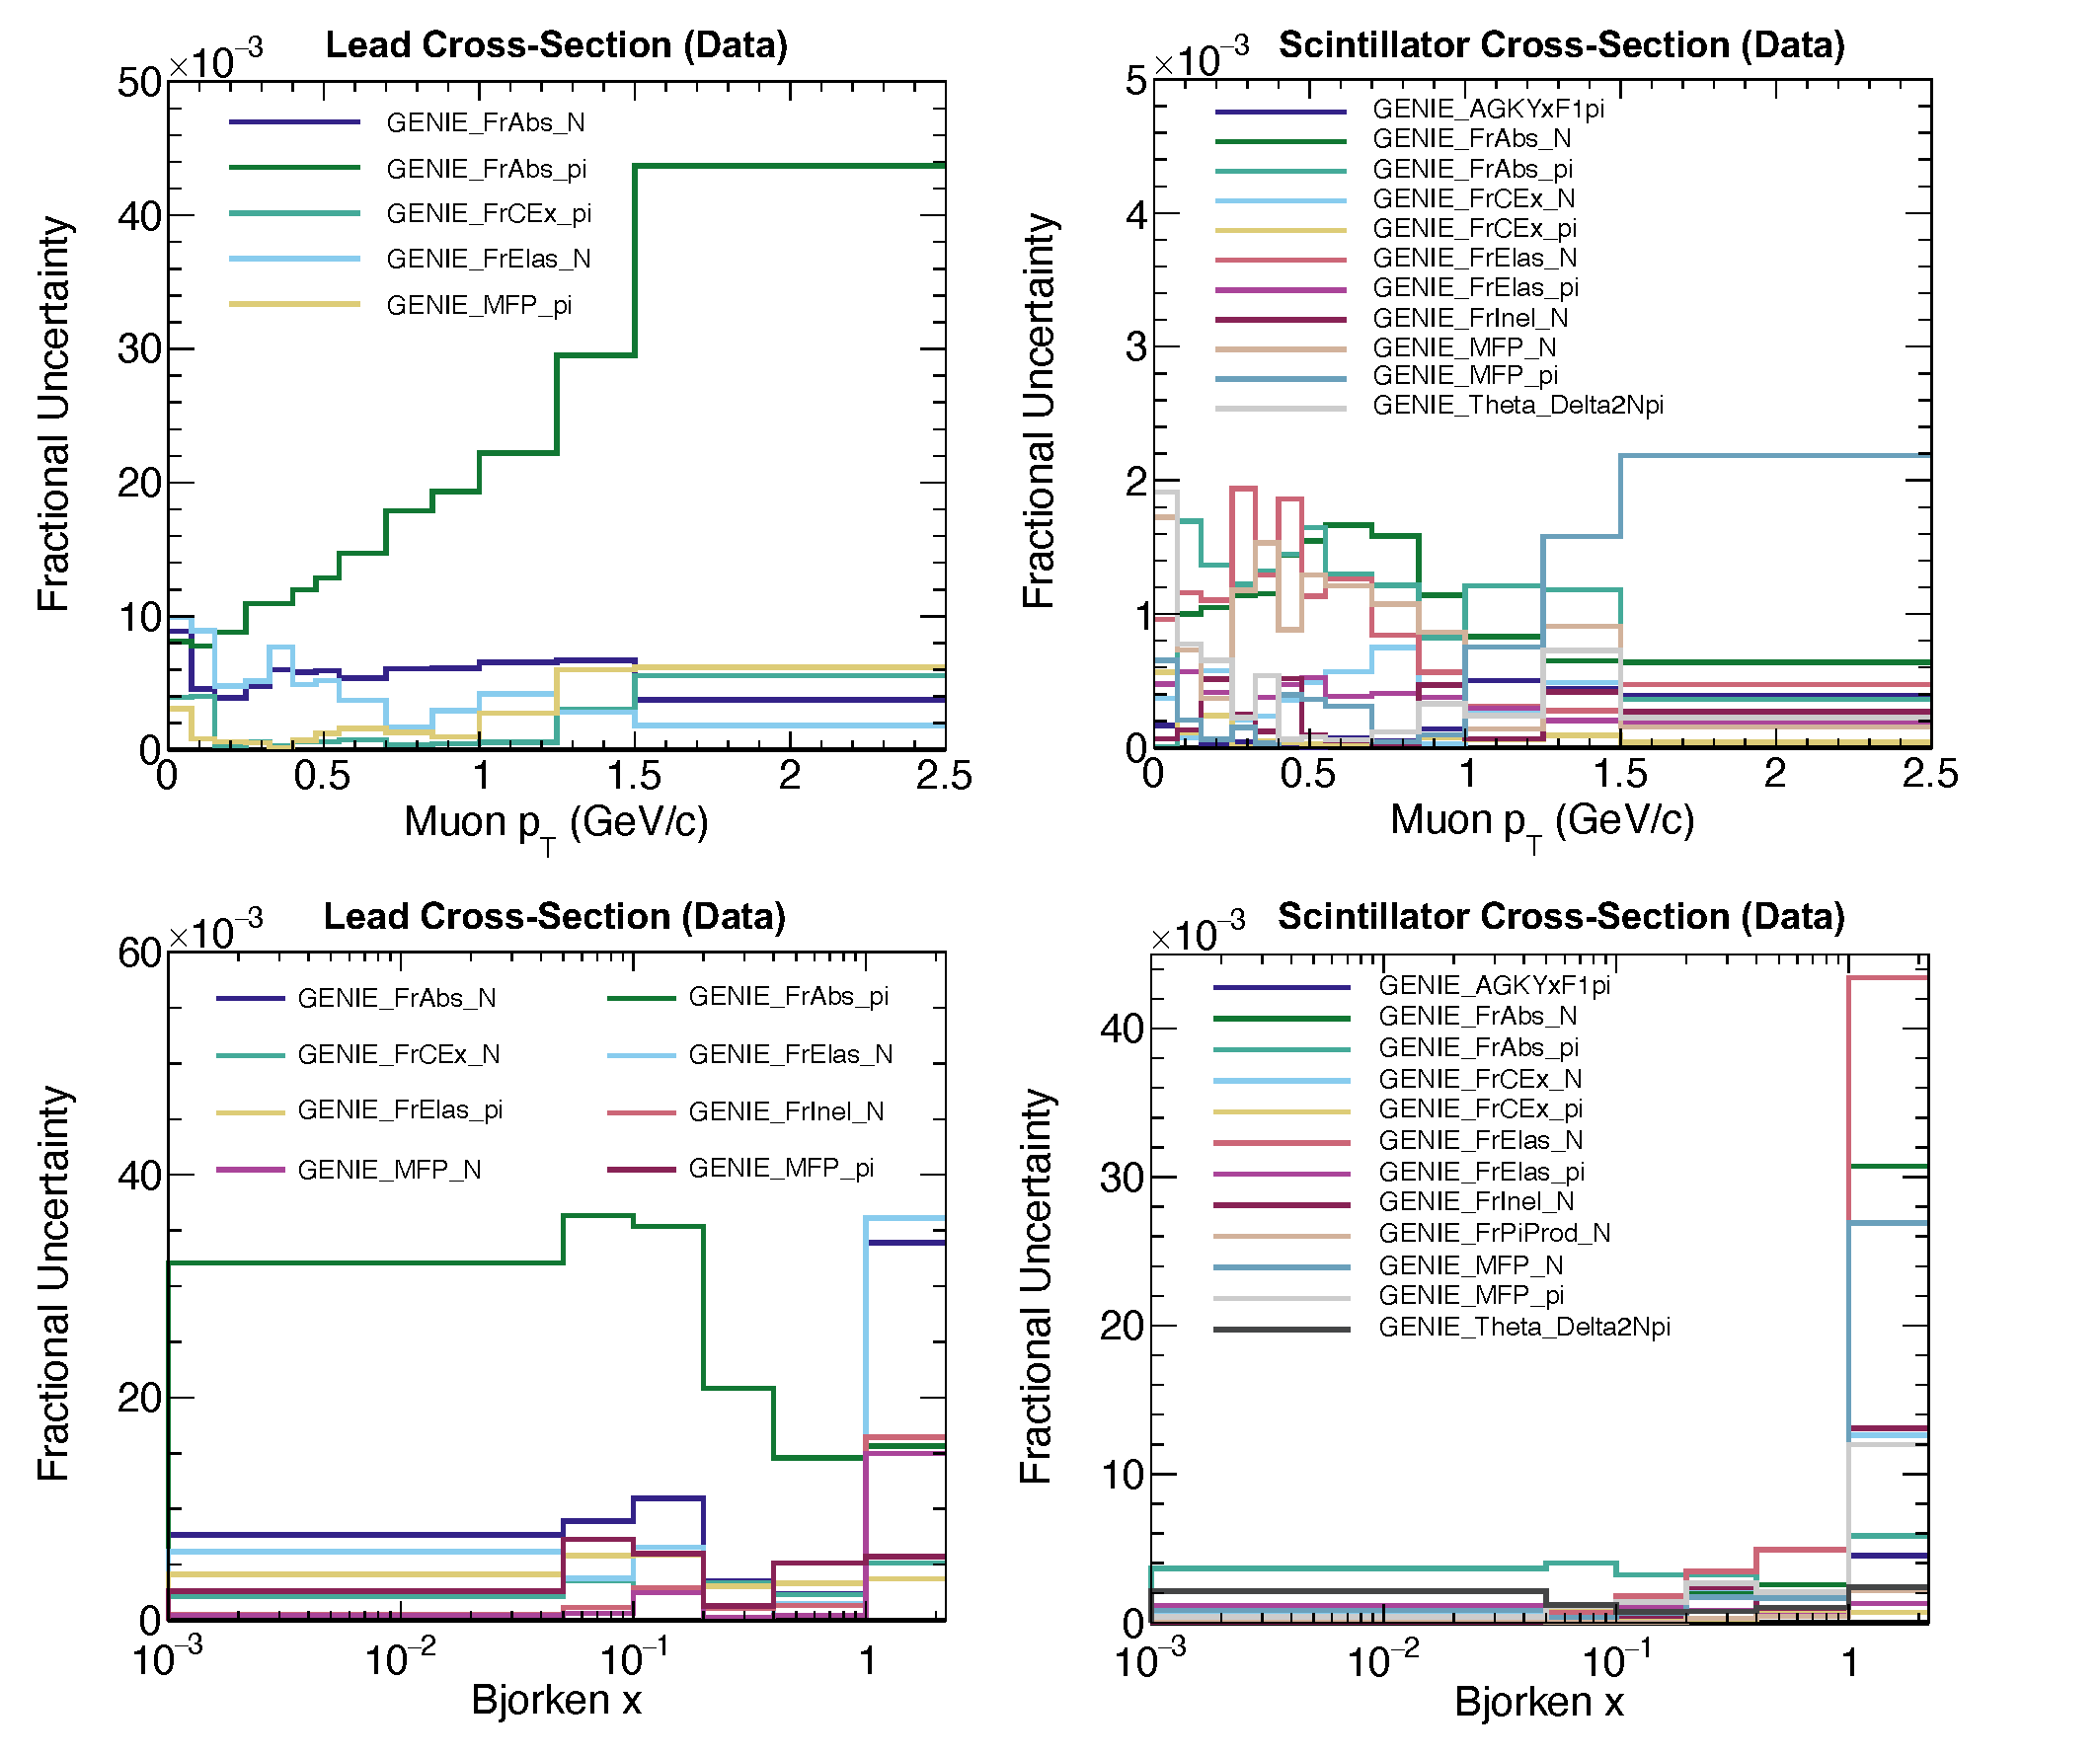
\includegraphics[width=1\textwidth]{08systematics/figures/fsi_t5leadTracker_pTx.pdf} }%
    \caption{Breakdown of various sources of uncertainty in the `FSI' error band of the differential cross-section in data, both in $p_{\text{T}}$ (top) and Bjorken $x$ (bottom) for lead (left panel) and scintillator (right panel). Note that only uncertainties that contribute more than 0.5\%  for lead and more than 0.05\% for scintillator are shown, illustrating the striking difference in the FSI uncertainty in heavier nuclei.}%
    \label{fig:fsi_t5leadTracker_pTx}
\end{figure}

The uncertainty on the final-state interactions (FSI) refers to the combination of uncertainties in GENIE parameters governing all interactions following the initial interaction. In this context, in addition to the uncertainties on the intranuclear cascade parameters, the `FSI' error band also includes uncertainties on hadronisation and delta resonance decay (which are technically not FSI). The uncertainties in these parameters implemented in GENIE were originally determined by the MINOS collaboration~\cite{dytman2008hadronic}.\enlargethispage{1\baselineskip} 

Figure~\ref{fig:fsi_t5leadTracker_pTx} displays uncertainties in the $p_{\text{T}}$ and Bjorken~$x$ differential cross-sections on lead and scintillator that contribute more than 0.5\% and more than 0.05\%, respectively, to the `FSI' uncertainty band. A close-up of the scintillator breakdown in Bjorken~$x$ in the $x<1$~region is included in Appendix~\ref{ch:appendix_sysUncertainties}. The comparison between the heavy lead and the light scintillator highlights the major difference in their respective `FSI' contributions. The larger `FSI' uncertainty in lead is associated with its complex nuclear environment, characterised by a significantly higher number of nucleons compared to the scintillator, which is primarily composed of carbon. In particular, the primary source of uncertainty contributing significantly to the `FSI' error band in lead is related to the uncertainty regarding the probability of a pion produced in the initial interaction being absorbed by the nuclear environment, resulting in it not exiting the nucleus. This is not unexpected as the pion production represents the dominant channel in this analysis. Table~\ref{table:FSIUnc} provides a list and description of all parameters associated with the uncertainties presented in Figure~\ref{fig:fsi_t5leadTracker_pTx}.

% What is xF https://www.phenix.bnl.gov/WWW/publish/seto/tutorials/notes%20on%20x_F%20and%20x_Bj%20for%20clarity.txt
% Note there was a bug in 2.12.6 in this (before this it was all isotropic) but not big impact at all on this analysis
% didn't fix it so it goes from anisotropic to more anisotropic
\begin{table}[b!]
    \centering
    \small
    \begin{tabularx}{1.0\textwidth}{c c L}
    \hline \\ [-1.5 ex]
    Error band & 1$\sigma$ & Description\\ [0.5ex] % inserts table %heading
    \hline
    \hline \\ [-2ex]
    AGKYxF1pi & $\pm20$\% & Modifies DIS hadronisation model for low multiplicity production of nucleons and pions \\
    FrAbs\_N & $\pm20$\% & Absorption probability for nucleons (for given total rescattering probability) \\
    FrAbs\_pi & $\pm30$\% & Absorption probability for pions (for given total rescattering probability) \\
    FrCEx\_N & $\pm50$\% & Charge exchange probability for nucleons (for given total rescattering probability)\\
    FrCEx\_pi & $\pm50$\% & Charge exchange probability for pions (for given total rescattering probability)\\
    FrElas\_N & $\pm30$\% & Elastic scattering probability for nucleons (for given total rescattering probability) \\
    FrElas\_N & $\pm10$\% & Elastic scattering probability for pions (for given total rescattering probability) \\
    FrInel\_N & $\pm40$\% & Inelastic scattering probability for nucleons (for given total rescattering probability) \\
    FrPiProd\_N & $\pm20$\% & Pion production probability for nucleons (for given total rescattering probability)\\
    MFP\_N &$\pm20$\%  & Modifies the mean free path for nucleons \\
    MFP\_pi & $\pm20$\% & Modifies the mean free path for pions \\
    Theta\_Delta2Npi & $\pm100$\% & Uncertainty on the anisotropy of the delta decay angular distribution \\
    \hline
    \end{tabularx}
    \caption{Description of various sources of uncertainty in the `FSI' error band from Figure~\ref{fig:fsi_t5leadTracker_pTx} with their corresponding 1$\sigma$ shifts.}
    \label{table:FSIUnc}
\end{table}

\section{Particle response}
%  no detector response uncertainty on muon variables (recoil reconstruction has no impact) in comparison to Bjorken x
% GEANT neutron modelling significant in both pT and Bjorken x - why?

\begin{figure}[b!]%
    \vspace{-7pt}
    \centering
   {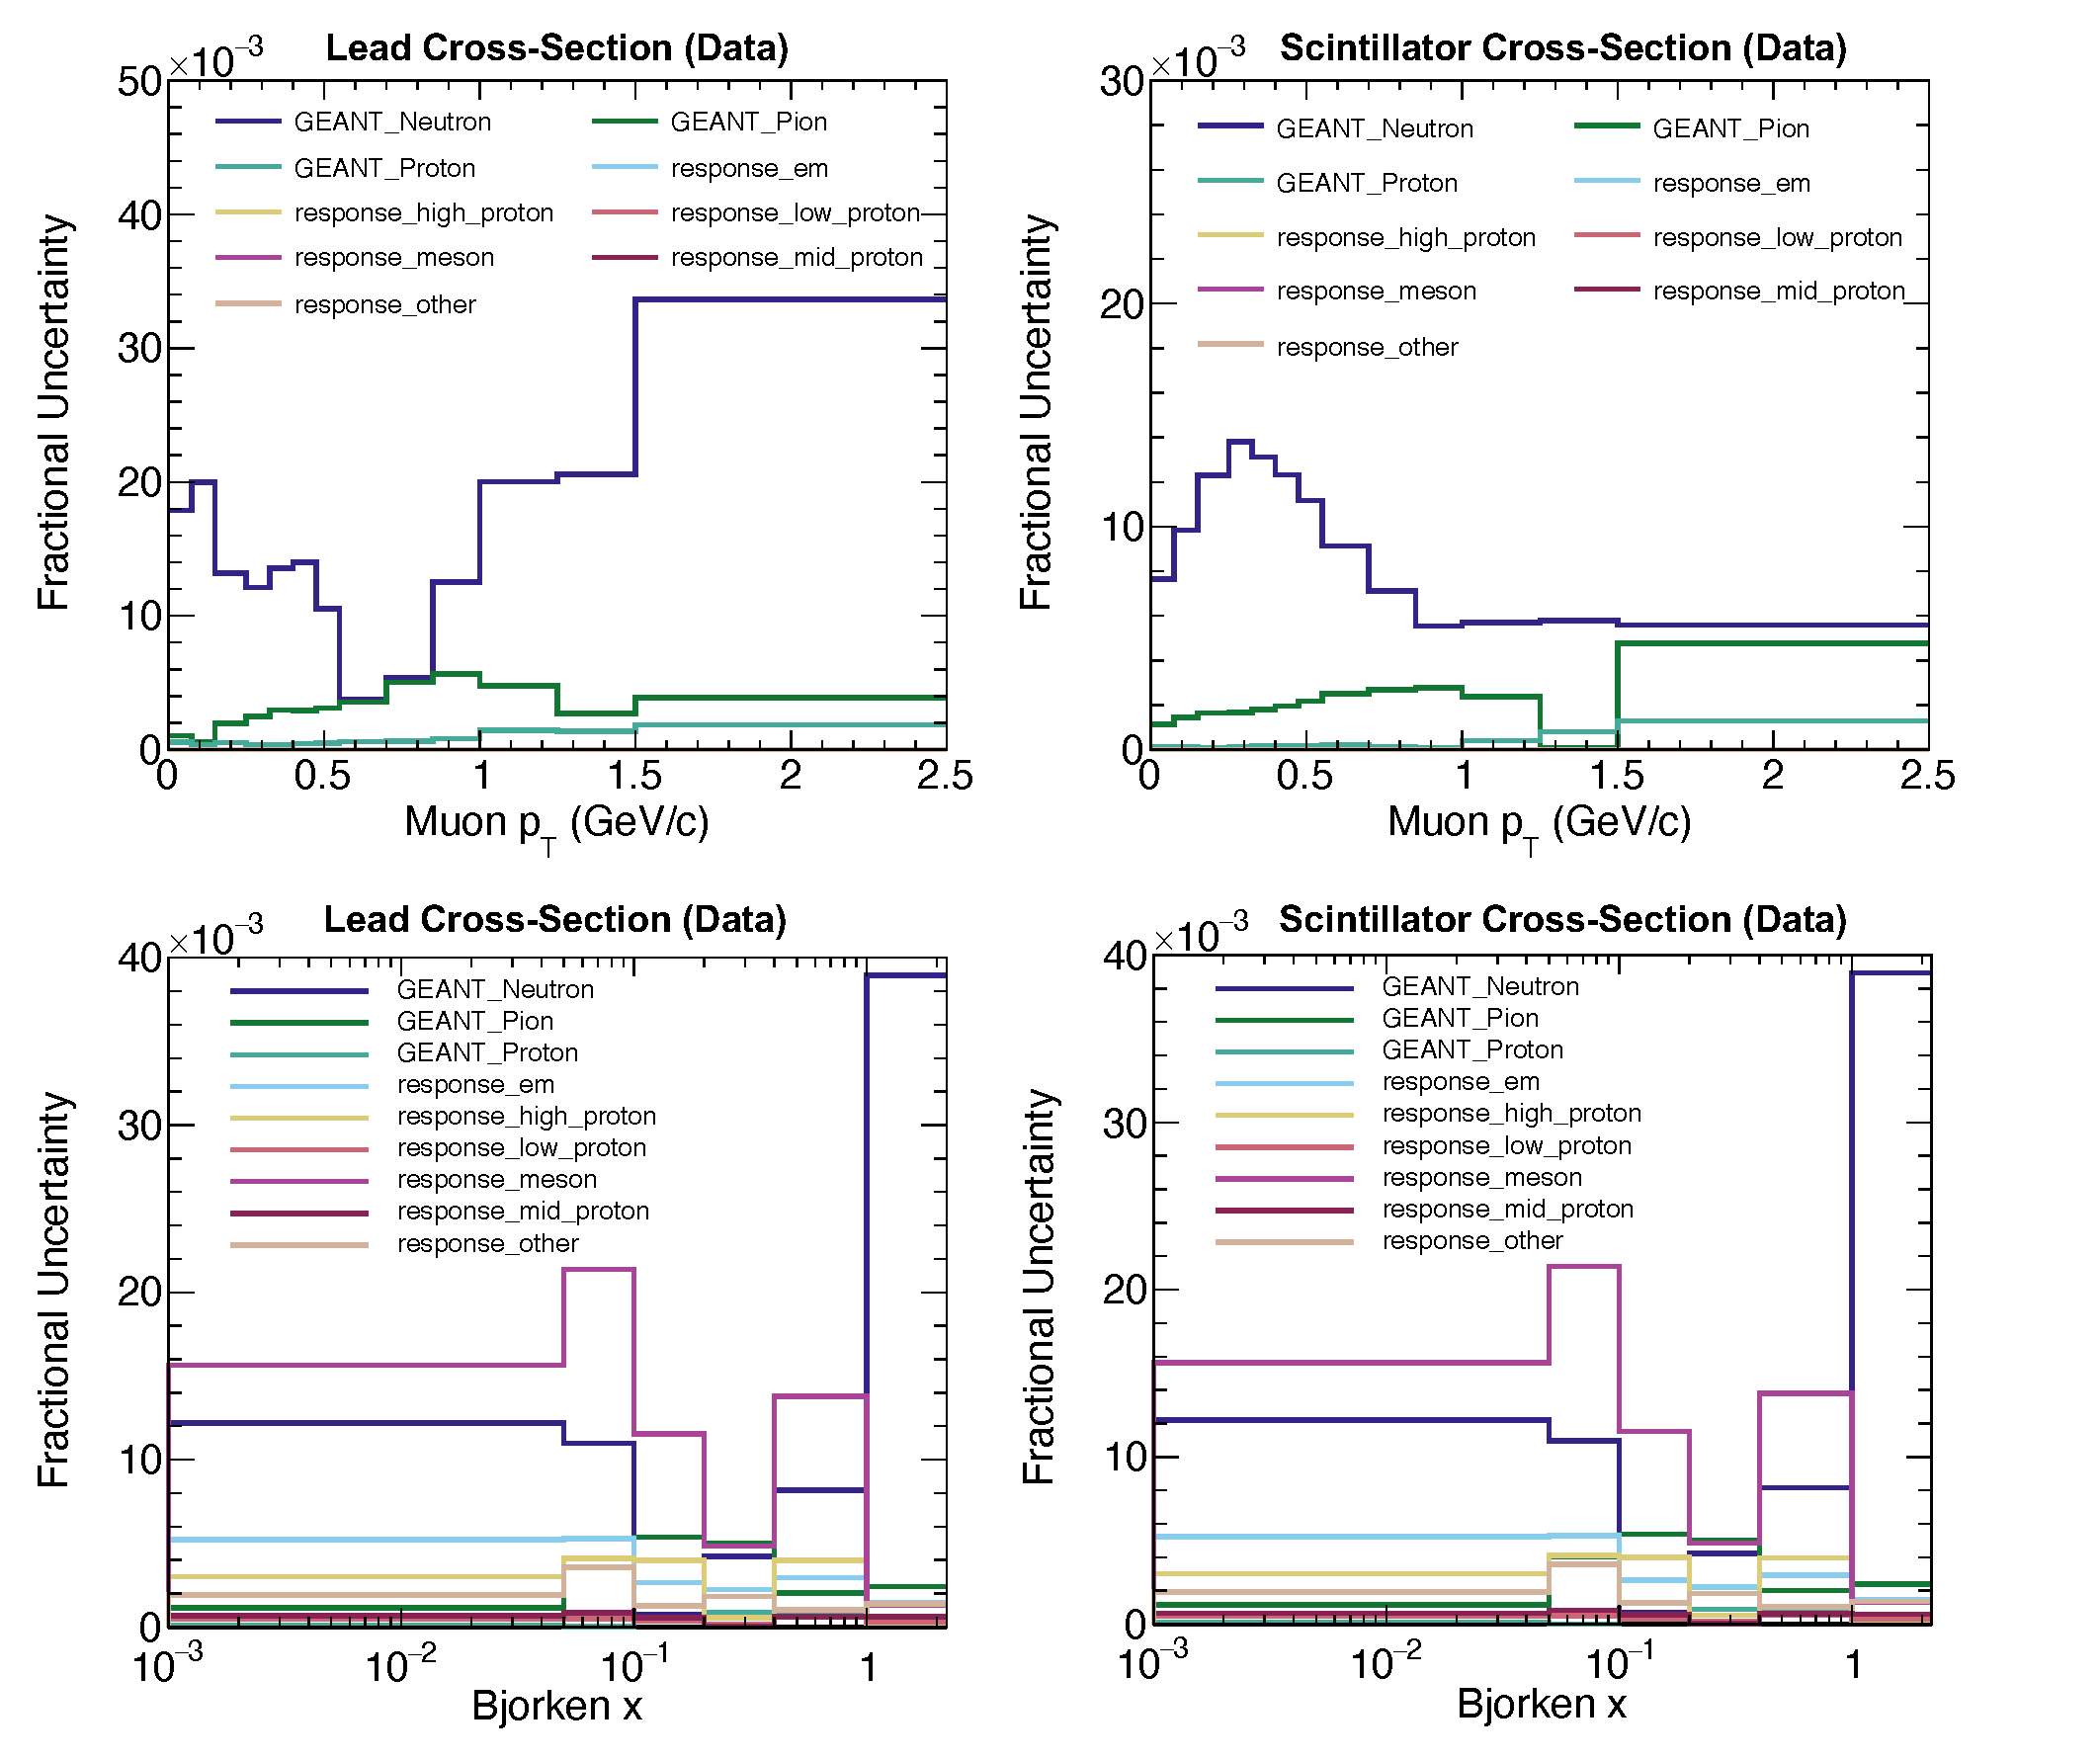
\includegraphics[width=1\textwidth]{08systematics/figures/response_t5leadTracker_pTx.pdf} }%
    \caption{Breakdown of various sources of uncertainty in the `Particle Response' error band of the differential cross-section in data, both in $p_{\text{T}}$ (top) and Bjorken $x$ (bottom) for lead (left panel) and scintillator (right panel). Note the additional contribution from uncertainties related to the calorimetric detector response relevant to recoil reconstruction in Bjorken $x$.}%
    \label{fig:response_t5leadTracker_pTx}
\end{figure}

The `Particle Response' error band in Figures~\ref{fig:mcSimulationFracUnc_t5lead_pTx} and~\ref{fig:crossSectionFracUnc_lead_pTx} includes uncertainties concerning both the interaction cross-sections used by GEANT4~\cite{Geant4_AGOSTINELLI2003250, Geant4_1610988} for simulating final-state particles as they traverse the MINERvA detector (discussed in Chapter~\ref{ch:dataAsimulation}) and the calorimetric detector response relevant to recoil reconstruction (described in Chapter~\ref{ch:Reconstruction}). Figure~\ref{fig:response_t5leadTracker_pTx} breaks down the sources of uncertainties contributing to this error band in the $p_{\text{T}}$ and Bjorken~$x$ differential cross-sections on lead and scintillator.\enlargethispage{1.\baselineskip} 

To evaluate the uncertainty associated with the GEANT4 simulation, MINERvA varies the hadronic inelastic cross-section of the final-state protons and pions based on the MINERvA test beam data~\cite{ALIAGA201528}~according to the procedure described in Subsection~\ref{sec:particleProp}. The uncertainty on the neutron inelastic cross-section reflects the reweight to the Abfalterer \textit{et al.}~data~\cite{Abfalterer_PhysRevC.63.044608} also outlined in Subsection~\ref{sec:particleProp}. The GEANT4 neutron uncertainty also accounts for the uncertainty on neutron energy deposits, as the neutron energy deposition is dependent on the neutron inelastic cross-section.
% https://minerva-docdb.fnal.gov/cgi-bin/sso/ShowDocument?docid=7532
% 10\% C carbon, 15\% iron, 20\% lead for protons and pions

% GEANT systematics: % Systematics!! For example, for total inelastic cross-section for protons and pions, the variation is 10\% in carbon and hydrocarbon, 15\% in iron and 20\% in lead. Similarly, the neutron interaction cross-section is reweighted 
%https://minerva-docdb.fnal.gov/cgi-bin/sso/RetrieveFile?docid=7532&filename=dytman-hadr-uncert-27apr12.pdf&version=2

The uncertainties on how the MINERvA detector responds to various calorimetric recoil energy deposits from protons~\cite{protonTestbeam} and pions~\cite{pionTestbeam} are also constrained by the test beam studies~\cite{ALIAGA201528}. The electromagnetic response uncertainty is derived from differences between data and simulation when observing Michel electrons (electrons from muon decay)~\cite{Aliaga_2014}. Other unconstrained contributions are assigned conservative uncertainties. All these uncertainties for various particle energy deposits are summarised in Table~\ref{table:responseUnc}.

The comparison between lead and scintillator in Figure~\ref{fig:response_t5leadTracker_pTx} highlights that uncertainties in the modelling of inelastic cross-sections are more pronounced for heavier targets. Overall, the uncertainty on neutron modelling is the largest, contributing significantly to both $p_{\text{T}}$ and Bjorken~$x$ distribution. In $p_{\text{T}}$ in particular, the effect is attributed to correlations between the outgoing particle kinematics, with $p_{\text{T}}$ serving as a proxy for the momentum transfer. Furthermore, as expected, uncertainties in the calorimetric response of the detector have a significant impact on the Bjorken~$x$ distribution, in contrast to the~$p_{\text{T}}$ distribution, which, by definition, does not depend on recoil reconstruction. Note that in Bjorken $x$, the dominant source of uncertainty corresponds to the detector's response to pions (mesons), consistent with pion production constituting the primary channel in this analysis. \enlargethispage{1.\baselineskip} 

\begin{table}[b!]
    \centering
    \small
    \begin{tabularx}{0.94\textwidth}{c c L}
    \hline \\ [-1.5 ex]
    Error band & 1$\sigma$ & Description\\ [0.5ex] % inserts table %heading
    \hline
    \hline \\ [-2.0ex]
    response\_low\_proton & $\pm4.0$\% & Proton kinetic energy $< 50$ MeV \\
    response\_mid\_proton & $\pm3.5$\%  & Proton kinetic energy between $50$ MeV and $100$ MeV\\
    response\_high\_proton & $\pm3.0$\%  & Proton kinetic energy $> 100$ MeV  \\
    response\_meson & $\pm5.0$\%  & Pion kinetic energy between $400$ MeV and $1.9$ GeV \\
    response\_em & $ \pm3.0$\%  & Electromagnetic shower  \\
    response\_other & $\pm20.0$\%  &  Other \\
    \hline
    \end{tabularx}
    \caption{Description of various sources of uncertainty related to the calorimetric detector response relevant to recoil reconstruction in the `Particle Response' error band from Figure~\ref{fig:response_t5leadTracker_pTx} with their corresponding 1$\sigma$ shifts.}
    \label{table:responseUnc}
\end{table}

\section{Other}
% - ML vertex and uncertainty on target mass

Other uncertainties considered in this analysis are related to the material mass and the machine-learning-based vertex reconstruction. Specifically, the estimated uncertainties on the fiducial masses due to density and thickness variations are represented by $\pm0.5$\% shifts for the carbon and lead mass, $\pm1.0$\% for the iron mass, and $\pm1.4$\% for the scintillator mass~\cite{Aliaga_2014}. The uncertainty associated with the ability to correctly resolve the vertex position using machine learning is set conservatively by $\pm1.0$\% shifts relative to the central value based on my studies of the differences between the data and the simulation in the plane prediction distributions for antineutrino interaction vertices~\cite{Klustova_MLsys}. The `Other' error band in Figures~\ref{fig:mcSimulationFracUnc_t5lead_pTx} and~\ref{fig:crossSectionFracUnc_lead_pTx} represents the combination of these two uncertainties above and contributes slightly over 1\% to the total uncertainty in the differential cross-section. 

\section{Additional sources of uncertainties}
%- uncertainty on the sideband fit scale factor - added in quadrature to the statistical + systematic uncertainty
%- neutron/missing energy uncertainty 

Two additional systematic uncertainties arising from two aspects of the analysis procedure described in Chapter~\ref{ch:analysis1D}~are under consideration for implementation. Specifically, an uncertainty is proposed to account for the disagreement between the data and simulation after the data-driven plastic sideband fit procedure, outlined in Section~\ref{sec:bkgSubtraction}. This proposed uncertainty is aimed at addressing discrepancies that are not, in some bins, fully covered by the current list of systematic uncertainties. Alternatively, the shape differences could be mitigated by introducing a bin-by-bin scale factor, potentially eliminating the need for this additional systematic uncertainty, which is further discussed in Chapter~\ref{ch:results}.

Additionally, another uncertainty could account for potential model bias in the Bjor\-ken~$x$ cross-section introduced by the neutron modelling corrections at the unfolding level suggested by the exploratory study in Section~\ref{sec:migration_unfolding}. This proposed uncertainty would address the differences observed in the $x > 1$ region when unfolding data using simulations with modified true invisible energy distributions, as shown in Figure~\ref{fig:maresCheck_invisECheck} in the relevant section.\enlargethispage{1.5\baselineskip} However, in order to do so, it is essential to examine and understand the magnitude of the variations in invisible energy first. 